\upaper{29}{УПРАВЛЯЮЩИЕ ВСЕЛЕНСКОЙ МОЩЬЮ}
\uminitoc{СЕМЬ ВЕРХОВНЫХ УПРАВЛЯЮЩИХ МОЩЬЮ}
\uminitoc{ВЕРХОВНЫЕ ЦЕНТРЫ МОЩИ}
\uminitoc{СФЕРА ДЕЯТЕЛЬНОСТИ ЦЕНТРОВ МОЩИ}
\uminitoc{ГЛАВНЫЕ ФИЗИЧЕСКИЕ РЕГУЛЯТОРЫ}
\uminitoc{ГЛАВНЫЕ ОРГАНИЗАТОРЫ СИЛЫ}
\author{Всеобщий Цензор}
\vs p029 0:1 Из всех вселенских личностей, имеющих отношение к регулированию межпланетных и межвселенских дел, меньше всего на Урантии знали об управляющих мощью и их партнёрах. О существовании ангелов и подобных категорий небесных существ ваши расы знали уже давно, но вам почти ничего не сообщалось об управляющих и регуляторах физической области. Даже сейчас мне позволено полностью раскрыть только последнюю из следующих трёх групп живых существ, имеющих отношение к управлению силой и регулированию энергии в главной вселенной:
\vs p029 0:2 \li{1.}Первичные Возникшие Главные Организаторы Силы.
\vs p029 0:3 \li{2.}Младшие Трансцендентальные Главные Организаторы Силы.
\vs p029 0:4 \li{3.}Управляющие Вселенской Мощью.
\vs p029 0:5 \pc Хотя я считаю невозможным изобразить индивидуальность различных групп управляющих, центров и регуляторов вселенской мощи, я надеюсь, что смогу объяснить кое\hyp{}что о сфере их деятельности. Они представляют собой уникальную группу живых существ, связанных с разумным регулированием энергии во всей большой вселенной. Включая верховных управляющих, они включают следующие основные подразделения:
\vs p029 0:6 \li{1.}Семь Верховных Управляющих Мощью.
\vs p029 0:7 \li{2.}Верховные Центры Мощи.
\vs p029 0:8 \li{3.}Главные Физические Регуляторы.
\vs p029 0:9 \li{4.}Управляющие Моронтийной Мощью.
\vs p029 0:10 \pc Верховные Управляющие Мощью и Центры существовали почти вечно, и, насколько нам известно, существа этой категории больше не создавались. Семь Верховных Управляющих были персонализированы Семью Главными Духами, а затем они сотрудничали со своими родителями в создании более десяти миллиардов партнёров. До появления управляющих мощью энергетические контуры пространства за пределами центральной вселенной находились под разумным наблюдением Главных Организаторов Силы Рая.
\vs p029 0:11 Обладая знаниями о материальных созданиях, ты можешь хотя бы по контрасту составить представление о духовных существах; однако смертному разуму очень трудно представить себе управляющих мощью. По плану постепенного восхождения к более высоким уровням существования ты не будешь соприкасаться ни с верховными управляющими, ни с центрами мощи. В некоторых редких случаях ты будешь иметь дело с физическими регуляторами, и будешь свободно работать с управляющими моронтийной мощью по достижении обительских миров. Эти Управляющие Моронтийной Мощью действуют настолько исключительно в моронтийном режиме локальных творений, что лучше всего рассказывать об их деятельности в разделе, относящемся к локальной вселенной.
\usection{СЕМЬ ВЕРХОВНЫХ УПРАВЛЯЮЩИХ МОЩЬЮ}
\vs p029 1:1 Семь Верховных Управляющих Мощью являются регуляторами физической энергии большой вселенной. Их создание Семью Главными Духами стало первым зарегистрированным случаем получения полуматериального потомства от чисто духовных предков. Когда Семь Главных Духов творят индивидуально, они порождают высокодуховных личностей ангельского порядка; когда они создают коллективно, они иногда производят эти высокие типы полуматериальных существ. Но даже эти квазифизические существа невидимы для ближнего зрения [short\hyp{}range vision]\fnst{Возможно, что имеется в виду ограниченность зрения смертных, а может быть и что\hyp{}то другое\ldots} смертных Урантии.
\vs p029 1:2 Верховных Управляющих Мощью всего семь и они идентичны по внешнему виду и функциям. Одного невозможно отличить от другого, кроме как тому Главному Духу, с которым каждый Управляющий находится в непосредственной связи и которому полностью подчиняется функционально. Таким образом, каждый из Главных Духов находится в вечном союзе с одним из своих коллективных потомков. Один и тот же управляющий всегда связан с одним и тем же Духом, и их рабочее сотрудничество приводит к уникальной ассоциации физических и духовных энергий, полуфизического существа и духовной личности.
\vs p029 1:3 Семь Верховных Управляющих Мощью располагаются на периферийном Рае, где их медленно циркулирующие присутствия указывают на местонахождение центра фокуса силы Главных Духов. Эти управляющие мощью действуют по отдельности в регулировании мощи и энергии сверхвселенных, но коллективно при управлении центральным творением. Они действуют из Рая, но поддерживают своё присутствие\fnst{Буквально <<поддерживают себя в качестве эффективных центров мощи>>.} в качестве эффективных центров мощи во всех подразделениях большой вселенной.
\vs p029 1:4 Эти могущественные существа являются физическими предками огромного множества центров мощи и, через них, физических регуляторов, разбросанных по семи сверхвселенным. Такие подчинённые организмы физического контроля в основном однородны, идентичны, за исключением дифференцированной тонировки [toning] каждого сверхвселенского корпуса. Чтобы изменить своё служение в сверхвселенной, им просто нужно вернуться в Рай для перетонировки [retoning]. Физическое творение в основном единообразно в управлении.
\usection{ВЕРХОВНЫЕ ЦЕНТРЫ МОЩИ}
\vs p029 2:1 Семь Верховных Управляющих Мощью не могут воспроизводиться индивидуально, но коллективно и в ассоциации с Семью Главными Духами они могут и воспроизводят~--- создают~--- других, подобных себе, существ. Таково происхождение Верховных Центров Мощи большой вселенной, которые функционируют в следующих семи группах:
\vs p029 2:2 \li{1.}Верховные Управляющие Центрами.
\vs p029 2:3 \li{2.}Центры Хавоны.
\vs p029 2:4 \li{3.}Центры сверхвселенных.
\vs p029 2:5 \li{4.}Центры локальных вселенных.
\vs p029 2:6 \li{5.}Центры созвездий.
\vs p029 2:7 \li{6.}Центры систем.
\vs p029 2:8 \li{7.}Неклассифицированные Центры.
\vs p029 2:9 \pc Эти центры мощи вместе с Верховными Управляющими Мощью являются существами, обладающими высокой степенью свободы воли и волевых действий. Все они наделены личностью Третьего Источника и обнаруживают неоспоримую волевую способность высокого порядка. Эти управляющие центры вселенской системы мощи наделены изысканным разумом; они представляют собой интеллект системы мощи большой вселенной и секрет метода управления разумом всей обширной сети разветвлённых функций Главных Физических Регуляторов и Управляющих Моронтийной Мощью.
\vs p029 2:10 \li{1.}\bibemph{Верховные Управляющие Центрами}. Эти семь равных партнёров Верховных Управляющих Мощью являются регуляторами главных энергетических контуров большой вселенной. Центр каждого управляющего центрами находится на одном из особых миров Семи Верховных Исполнителей, и они работают в тесном сотрудничестве с этими координаторами общих вселенских дел.
\vs p029 2:11 Верховные Управляющие Мощью и Верховные Управляющие Центрами действуют как индивидуально, так и совместно в отношении всех космических явлений ниже уровней <<энергии гравитации>>. Действуя сообща, эти 14 существ являются для вселенской мощи тем же, чем Семь Верховных Исполнителей~--- для общих вселенских дел, а Семь Главных Духов~--- для космического разума.
\vs p029 2:12 \li{2.}\bibemph{Центры Хавоны}. До создания вселенных времени и пространства центры мощи не требовались в Хавоне, но с тех давних пор в центральном творении функционирует 1\,000\,000 центров, каждый из которых контролирует 1\,000 миров Хавоны. Здесь, в божественной вселенной, имеет место совершенство энергетического контроля~--- условие, не существующее где\hyp{}либо ещё. Совершенство регулирования энергии есть конечная цель всех центров мощи и физических регуляторов пространства.
\vs p029 2:13 \li{3.}\bibemph{Центры сверхвселенных}. Тысяча центров мощи третьего порядка занимают огромную площадь, располагаясь на столичной сфере каждой из семи сверхвселенных. Три тока первичной энергии, по 10 сегрегаций в каждом, подходят к этим центрам мощи, но 7 специализированных и точно направленных, хотя и несовершенно управляемых, контуров мощи исходят из области их совместного действия. Это~--- электронная организация вселенской мощи.
\vs p029 2:14 Вся энергия заключена в контур в цикле Рая, но Управляющие Вселенской Мощью \bibemph{управляют} силами\hyp{}энергиями нижнего Рая, в том виде, в каком они находят их~--- модифицированными в пространственных функциях центральной вселенной и сверхвселенных,~--- преобразовывая и направляя эти энергии в каналы полезного и конструктивного применения. Есть разница между энергией Хавоны и энергиями сверхвселенных. Заряд мощи сверхвселенной состоит из трёх фаз энергии по 10 сегрегаций в каждой. Этот тройной энергетический заряд распространяется по всему пространству большой вселенной; он подобен огромному движущемуся океану энергии, который целиком поглощает и омывает каждое из семи сверхтворений.
\vs p029 2:15 Электронная организация вселенской мощи функционирует в семи фазах и обнаруживает переменную реакцию на локальную или линейную гравитацию. Этот семичастный контур исходит из центров мощи сверхвселенных и пронизывает каждое сверхтворение. Такие специализированные токи времени и пространства представляют собой определённые и локализованные движения энергии, инициированные и направленные для конкретных целей, подобно тому, как Гольфстрим функционирует как ограниченное явление посреди Атлантического океана.
\vs p029 2:16 \li{4.}\bibemph{Центры локальных вселенных}. На столице каждой локальной вселенной размещено 100 центров силы четвёртого порядка. Они действуют, чтобы ослабить и иначе изменять семь контуров мощи, исходящих из столицы сверхвселенной, тем самым делая их пригодными для нужд созвездий и систем. Локальные астрономические катаклизмы пространства имеют для этих центров мощи преходящее значение; они занимаются организованной подачей полезной энергии дочерним созвездиям и системам. Они оказывают огромную помощь Сынам Создателям в более поздние времена организации вселенной и мобилизации энергии. Эти центры могут обеспечивать усиленные энергетические трассы, используемые для межпланетной связи между важными населёнными пунктами. Такая \bibemph{трасса,} или \bibemph{линия} энергии, иногда также называемая энергетическим путём, представляет собой прямой контур энергии от одного центра мощи к другому центру мощи или от одного физического регулятора к другому регулятору. Это~--- индивидуализированный поток мощи, в противоположность движениям недифференцированной энергии в свободном пространстве.
\vs p029 2:17 \li{5.}\bibemph{Центры созвездий}. По десять этих живых энергетических центров размещены в каждом созвездии; они функционируют как излучатели энергии для 100 подчинённых локальных систем. От этих существ исходят линии мощи для связи и транспортировки, а также для подпитки тех живых существ, которые зависят от определённых форм физической энергии для поддержания жизни. Но ни центры мощи, ни подчинённые им физические регуляторы в остальном не имеют отношения к жизни как функциональной организации.
\vs p029 2:18 \li{6.}\bibemph{Центры систем}. В каждую локальную систему постоянно назначается один Верховный Центр Мощи. Эти центры систем посылают контуры мощи в обитаемые миры времени и пространства. Они координируют деятельность подчинённых физических регуляторов и иным образом функционируют для обеспечения удовлетворительного распределения мощи в локальной системе. Передача энергии между планетами зависит от совершенной координации определённых материальных энергий и от эффективного регулирования физической мощи.
\vs p029 2:19 \li{7.}\bibemph{Неклассифицированные Центры}. Это~--- центры, которые действуют в особых локальных условиях, но не на обитаемых планетах. Индивидуальные миры находятся в ведении Главных Физических Регуляторов и получают входящие в контур линии мощи, передаваемые центром мощи их системы. Только у сфер, обладающих самыми необычными энергетическими взаимоотношениями, имеются центры мощи седьмого порядка, действующие как вселенские балансиры, или регуляторы энергии. В каждой фазе деятельности эти центры мощи полностью равны тем, которые действуют на более высоких единицах управления, но даже одно космическое тело из миллиона не является убежищем такой живой системы мощи.
\usection{СФЕРА ДЕЯТЕЛЬНОСТИ ЦЕНТРОВ МОЩИ}
\vs p029 3:1 Верховных Центров Мощи, распределённых по всем сверхвселенным, вместе с партнёрами и подчинёнными, свыше десяти миллиардов. И все они находятся в совершенной синхронности и полной связи со своими Райскими прародителями, Семью Верховными Управляющими Мощью. Таким образом, контроль мощи большой вселенной возложен на Семь Главных Духов, создателей Семи Верховных Управляющих Мощью.
\vs p029 3:2 Верховные Управляющие Мощью и все их партнёры, помощники и подчинённые навсегда освобождены от задержания или вмешательства со стороны всех трибуналов всего пространства; не подчиняются они и административному руководству сверхвселенского правительства От Века Древних или правительств Сынов Создателей локальных вселенных.
\vs p029 3:3 Эти центры и управляющие мощью созданы детьми Бесконечного Духа. Они не имеют отношения к администрации Сынов Бога, хотя и присоединяются к Сынам Создателям в более поздние эпохи материальной организации вселенной. Но центры мощи неким образом тесно связаны с космическим сверхуправлением Верховного Существа.
\vs p029 3:4 \pc Центры мощи и физические регуляторы не проходят никакого обучения; все они созданы в совершенстве и от природы совершенны в действии. Они никогда не переходят от одной функции к другой; они всегда служат в изначальном назначении. В их рядах нет развития, и это верно касательно всех семи подразделений обоих категорий.
\vs p029 3:5 Не имея связанного с восхождением прошлого, к которому можно было бы возвращаться в памяти, центры мощи и физические регуляторы никогда не развлекаются; во всех своих действиях они ведут себя исключительно по\hyp{}деловому. Они всегда на службе; во всеобщем плане не предусмотрено прерывание физических линий энергии; никогда, ни на долю секунды эти существа не могут оставить своё прямое наблюдение за энергетическими контурами времени и пространства.
\vs p029 3:6 \pc Управляющие, центры и регуляторы мощи не имеют отношения ни к чему во всём творении, кроме мощи~--- материальной или полуфизической энергии; они не порождают её, а модифицируют, манипулируют и направляют. Они также не имеют никакого отношения к физической гравитации, кроме сопротивления её притягивающей силе. Их отношение к гравитации полностью отрицательное.
\vs p029 3:7 Центры мощи используют обширные механизмы и согласования материального типа в связи с живыми механизмами различных сегрегированных концентраций энергии. Каждый индивидуальный центр мощи состоит ровно из 1\,000\,000 единиц функционального контроля, и эти энергомодифицирующие единицы не являются стационарными, подобно жизненно важным органам физического тела человека; <<жизненно важные органы>> регуляции мощи подвижны и поистине калейдоскопичны\fnst{То есть обладают различными возможностями в зависимости от их сочетаний.} по ассоциативным возможностям.
\vs p029 3:8 Я совершенно неспособен объяснить, каким образом эти живые существа охватывают собой манипулирование и регулирование главных контуров вселенской энергии. Дальнейшая попытка проинформировать тебя касательно размеров и функций этих гигантских и почти совершенно эффективных центров мощи вызвала бы у тебя ещё б\'ольшую растерянность и ужас. Они и живые, и <<личностные>>, но находятся за пределами возможностей твоего понимания.
\vs p029 3:9 \pc За пределами Хавоны Верховные Центры Мощи функционируют только на специально сконструированных (архитектурных) сферах или на других подходящим образом устроенных космических телах. Архитектурные миры устроены так, что живые центры мощи могут действовать как селективные переключатели, чтобы направлять, изменять и концентрировать энергии пространства, изливающиеся на эти сферы. Они не могли бы так функционировать на обычном эволюционном солнце или планете. Некоторые группы также занимаются обогревом и другими материальными потребностями этих специальных столичных миров. И хотя это выходит за рамки знания на Урантии, я могу заявить, что эти категории живых личностей мощи имеют много общего с распределением света, который светит без тепла\fnst{В физике принято называть <<светом без тепла>> различные виды люминесценции.}. Они не создают это явление, но они связаны с его распространением и направлением.
\vs p029 3:10 \pc Центры мощи и подчинённые им регуляторы назначаются на обработку всех видов физических энергий организованного пространства. Они работают с тремя основными токами по десять видов энергий в каждом. Это~--- энергетический заряд организованного пространства, а организованное пространство является их сферой деятельности. Управляющие Вселенской Мощью не имеют абсолютно никакого отношения к тем колоссальным силовым действиям, которые сейчас происходят за пределами нынешних границ семи сверхвселенных.
\vs p029 3:11 Центры и регуляторы мощи осуществляют совершенный контроль только над семью из десяти форм энергии, содержащихся в каждом основном вселенском токе; те формы, которые частично или полностью освобождены от их контроля, должно быть представляют собой непредсказуемые области проявления энергии, в которых доминирует Безусловный Абсолют. Если они и оказывают влияние на изначальные силы этого Абсолюта, нам об этом не известно, хотя есть некоторые незначительные свидетельства в пользу того мнения, что определённые физические регуляторы иногда автоматически реагируют на определённые импульсы Универсального Абсолюта.
\vs p029 3:12 Эти живые механизмы мощи не связаны сознательно с энергетическим сверхуправлением Безусловного Абсолюта в главной вселенной, но мы предполагаем, что вся их почти совершенная схема управления мощью каким\hyp{}то неизвестным образом подчинена этому надгравитационному присутствию. В любой локальной энергетической ситуации центры и регуляторы проявляют почти верховность, но они всегда осознают надэнергетическое присутствие и нераспознаваемые действия Безусловного Абсолюта.
\usection{ГЛАВНЫЕ ФИЗИЧЕСКИЕ РЕГУЛЯТОРЫ}
\vs p029 4:1 Эти существа являются мобильными подчинёнными Верховных Центров Мощи. Физические регуляторы наделены способностью метаморфозы индивидуальности такого рода, что они могут участвовать в удивительном разнообразии самопереноса, будучи способны пересекать локальное пространство со скоростями, приближающимися к скорости полёта Одиноких Посланников. Но подобно всем другим пересекающим пространство существам, они нуждаются в помощи как своих собратьев, так и некоторых других типов существ для преодоления действия гравитации и сопротивления инерции при отправке с материальной сферы.
\vs p029 4:2 Главные Физические Регуляторы служат по всей большой вселенной. Они непосредственно управляются из Рая Семью Верховными Управляющими Мощью вплоть до столиц сверхвселенных; отсюда они направляются и распределяются Советом Равновесия, высокоуполномоченными по мощи, посланными Семью Главными Духами из персонала Младших Главных Организаторов Силы. Эти высокоуполномоченные вправе интерпретировать показания и индикации главных франдаланков~--- живых инструментов, которые показывают напряжение мощи и энергетический заряд всей сверхвселенной.
\vs p029 4:3 В то время как присутствие Райских Божеств окружает большую вселенную и развёртывается по кругу вечности, влияние любого из Семи Главных Духов ограничено одной сверхвселенной. Существует чёткая сегрегация энергии и разделение контуров мощи между семью сверхтворениями; поэтому должны преобладать и преобладают индивидуализированные методы контроля.
\vs p029 4:4 \pc Главные Физические Регуляторы являются прямым потомством Верховных Центров Мощи, и в их число входят следующие:
\vs p029 4:5 \li{1.}Младшие Управляющие Мощью.
\vs p029 4:6 \li{2.}Механические регуляторы.
\vs p029 4:7 \li{3.}Преобразователи энергии.
\vs p029 4:8 \li{4.}Передатчики энергии.
\vs p029 4:9 \li{5.}Первичные ассоциаторы.
\vs p029 4:10 \li{6.}Вторичные диссоциаторы.
\vs p029 4:11 \li{7.}Франдаланки и хронолдеки.
\vs p029 4:12 \pc Не все эти категории~---личности в смысле обладания индивидуальной свободой выбора. Особенно последние четыре кажутся полностью автоматическими и механическими в реакции на импульсы вышестоящих и существующие энергетические условия. Но хотя такая реакция кажется полностью механической, это не так; они могут казаться автоматами, но все они раскрывают характерную функцию интеллекта.\tunemarkup{pictures}{\begin{figure}[H]\centering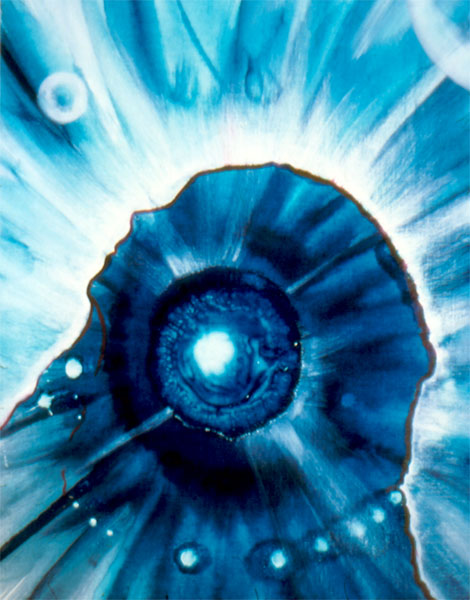
\includegraphics[width=0.82\columnwidth]{images/Morontia-Soul.jpg}\caption{Моронтийная душа, Винсент Вентола.}\end{figure}}
\vs p029 4:13 Личность не обязательно сопутствует разуму. Разум может мыслить даже если он полностью лишён способности выбора, как это наблюдается у многочисленных низших типов животных и у некоторых из этих подчинённых физических регуляторов. Многие из этих более автоматических регуляторов физической мощи не являются личностями ни в каком смысле этого слова. Они не наделены волей и способностью принимать независимые решения, будучи полностью подчинёнными механическому совершенству конструкции для задач, которые на них возложены. Тем не менее все они являются высокоразумными существами.
\vs p029 4:14 Физические регуляторы в основном заняты настройкой основных энергий, не открытых на Урантии. Эти неизвестные энергии очень важны для межпланетной системы транспорта и для некоторых способов связи. Когда мы прокладываем линии энергии с целью передачи эквивалентов звука или расширения зрения, эти неоткрытые формы энергии используются живыми физическими контролерами и их партнёрами. Эти же энергии иногда используются промежуточными созданиями в их повседневной работе\fnst{Действительно, при контактах с серафимами при поддержке промежуточных созданий происходит расширение зрения за пределы обычной октавы видимого света. В этой связи любопытно отметить следующий факт: при расширении зрения для восприятия формы серафима (например, в виде красного огненного столба) или формы моронтийной души (в виде голубого пульсирующего шара в области между горлом и солнечным сплетением, с нитями и <<клубами дыма>> внутри), все окружающие материальные предметы представляются в \bibemph{чёрно\hyp{}белой} форме, тогда как предметы из <<расширенной области>> видны в \bibemph{цвете}.}.\tunemarkup{pictures}{\begin{figure}[H]\centering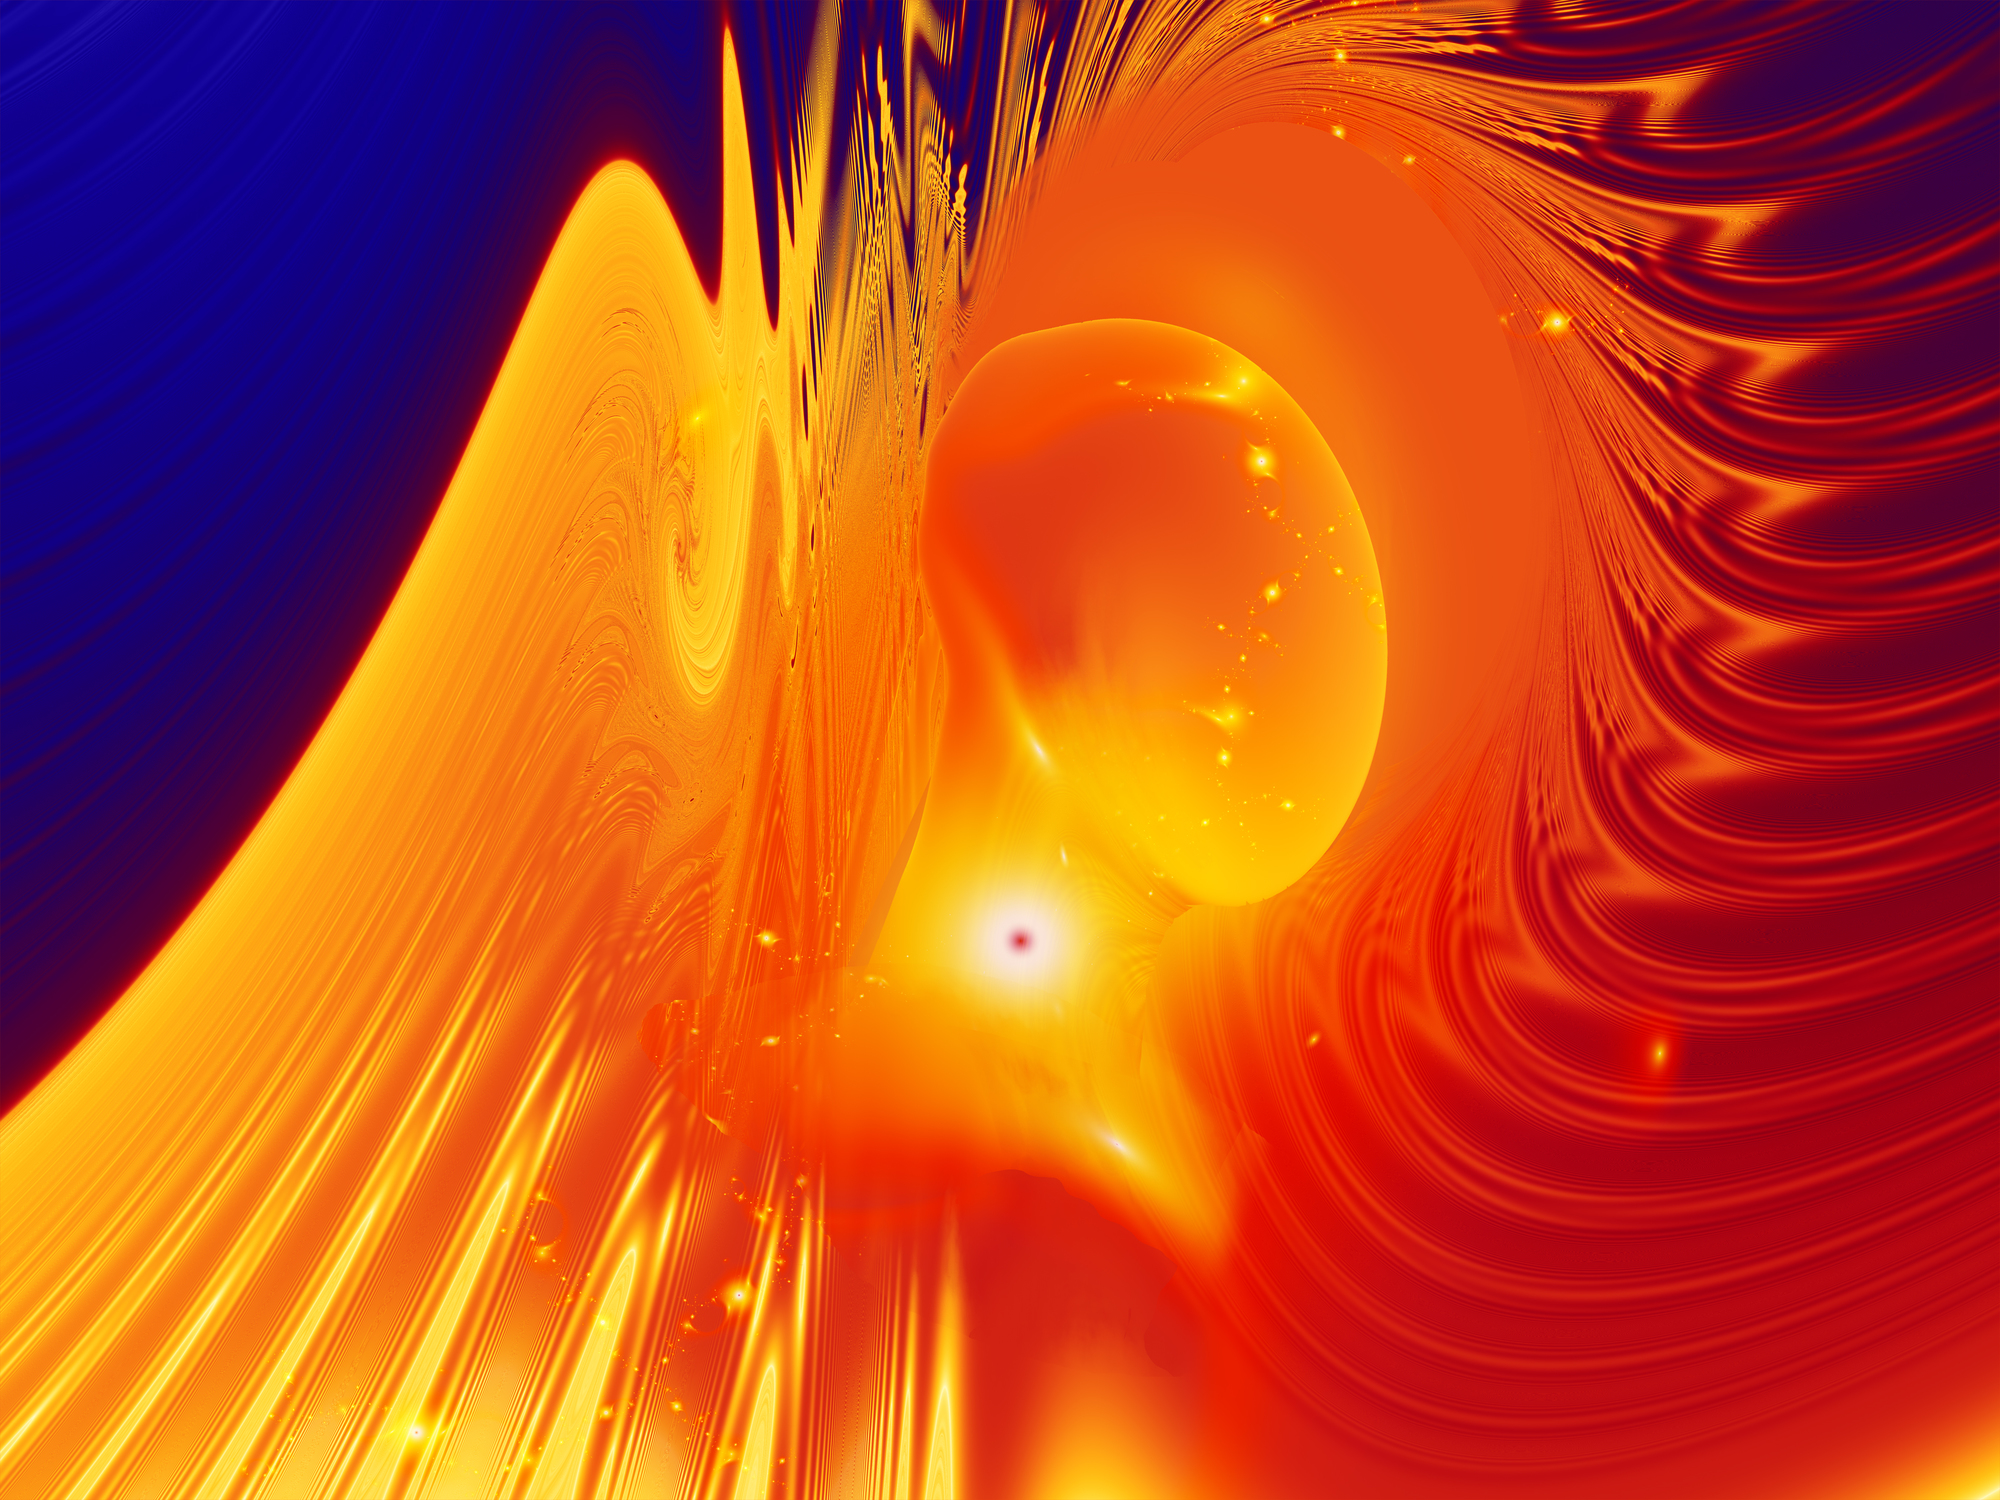
\includegraphics[width=0.95\columnwidth]{images/Seraphim.jpg}\caption{Серафим, Трой Бишоп.}\end{figure}}
\vs p029 4:15 \li{1.}\bibemph{Младшие Управляющие Мощью}. Этим удивительно эффективным существам доверено назначение и отправка всех категорий Главных Физических Регуляторов в соответствии с постоянно меняющимися потребностями постоянно изменяющегося энергетического статуса миров. Огромные резервы физических регуляторов поддерживаются на столичных мирах малых секторов, и из этих концентрационных пунктов они периодически отправляются младшими управляющими мощью в столицы вселенных, созвездий и систем, а также на отдельные планеты. Получив такое назначение, физические регуляторы временно подчиняются приказам божественных исполнителей миротворческих комиссий, но в остальном подчиняются исключительно своим помощникам управляющим и Верховным Центрам Мощи.
\vs p029 4:16 В каждый из малых секторов Орвонтона назначено 3\,000\,000 младших управляющих мощью, что в сумме составляет 3\,000\,000\,000 в качестве сверхвселенской квоты этих удивительно разносторонних существ. Их собственные резервы содержатся на тех же самых мирах малых секторов, где они служат также в качестве инструкторов для всех, кто изучает науки о методах интеллектуального контроля и трансмутации энергии.
\vs p029 4:17 Эти управляющие чередуют периоды исполнительной службы в малых секторах с равными периодами инспекционной службы в мирах пространства. Хотя бы один действующий инспектор всегда присутствует в каждой локальной системе, поддерживая центр на её столичной сфере. Они поддерживают гармоничную синхронизацию всего обширного скопления живой энергии.
\vs p029 4:18 \li{2.}\bibemph{Механические регуляторы}. Это чрезвычайно разносторонние и мобильные помощники младших управляющих мощью. Триллионы и триллионы их посылаются в Энсу, ваш малый сектор. Эти существа называются механическими регуляторами, потому что они полностью подвластны своим вышестоящим, целиком подчинены воле младших управляющих мощью. Тем не менее они сами по себе весьма умны, и их работа, хотя и механическая и прозаичная по природе своей, выполняется умело.
\vs p029 4:19 Из всех Главных Физических Регуляторов, назначенных в обитаемые миры, механические регуляторы безусловно являются самыми могущественными. Обладая живым даром антигравитации, больше всех других существ, каждый регулятор обладает сопротивлением гравитации, сравнимым только с сопротивлением гигантских сфер, вращающихся с огромной скоростью. Десять из этих регуляторов в настоящее время несут службу на Урантии, и одним из важнейших видов их планетарной деятельности является содействие отправлению серафических транспортов. При выполнении этой функции все 10 механических регуляторов действуют в унисон, в то время как батарея из 1\,000 передатчиков энергии обеспечивает начальный импульс для отправления серафима.
\vs p029 4:20 Механические регуляторы способны направлять поток энергии и способствовать её концентрации в специализированных токах или контурах. Эти могущественные существа непосредственно связаны с сегрегацией, направлением и усилением физических энергий и с уравновешиванием напряжений межпланетных контуров. Они являются экспертами в управлении 21 из 30 физических энергий пространства, составляющих энергетический заряд сверхвселенной. Им также удаётся добиться многого в управлении и контроле над 6 из 9 более тонких форм физической энергии. Помещая этих регуляторов в подходящем техническом отношении друг с другом и с определёнными центрами мощи, младшие управляющие мощью получают возможность производить невероятные изменения в настройке мощи и управлении энергией.
\vs p029 4:21 Главные Физические Регуляторы часто действуют в батареях из сотен, тысяч и даже миллионов, и, изменяя своё положение и построение, могут управлять энергией как коллективно, так и индивидуально. По мере изменения требований они могут повышать и ускорять объём и движение энергии или задерживать, конденсировать и замедлять энергетические токи. Они влияют на преобразования энергии и мощи подобно так называемым катализаторам, усиливающим химические реакции. Они функционируют благодаря врождённым способностям и в сотрудничестве с Верховными Центрами Мощи.
\vs p029 4:22 \li{3.}\bibemph{Преобразователи энергии}. Число этих существ в сверхвселенной невероятно велико. Только в одной Сатании их почти 1\,000\,000, а обычная квота составляет 100 на каждый обитаемый мир.
\vs p029 4:23 Преобразователи энергии являются совместным творением Семи Верховных Управляющих Мощью и Семи Управляющих Центрами\fnst{В тексте первого издания 1955 года <<Seven Central Supervisors>>, то есть <<Семь Центральных Управляющих>>, но текст был изменён на <<Seven Centre Supervisors>>, ибо последние известны из \bibref[29:2.10]{p029 2:10}, а первые нигде больше не упоминаются.}. Они относятся к числу более личностных категорий физических регуляторов, и за исключением тех случаев, когда на обитаемом мире присутствует младший управляющий мощью, руководство осуществляют преобразователи. Они являются планетарными инспекторами всех отбывающих серафических транспортов. Все классы небесной жизни могут использовать менее личностные категории физических регуляторов только посредством связи с более личностными категориями младших управляющих и преобразователей энергии.
\vs p029 4:24 Эти преобразователи представляют собой мощные и эффективные живые переключатели, будучи в состоянии располагаться по или против данного расположения или направления мощи. Они также искусно изолируют планеты от мощных потоков энергии, проходящих между гигантскими планетарными и звёздными соседями. Способность преобразовывать энергию делает их наиболее полезными в важной задаче поддержания всеобщего энергетического баланса или равновесия мощи. В какие\hyp{}то моменты кажется, что они потребляют или накапливают энергию; в другие,~--- что они источают или высвобождают энергию. Преобразователи способны увеличивать или уменьшать <<аккумуляторный>> потенциал живых и мёртвых энергий в соответствующих им областях. Но они имеют дело только с физическими и полуматериальными энергиями, они не функционируют непосредственно в сфере жизни, как не меняют они и формы живых существ.
\vs p029 4:25 В некоторых отношениях преобразователи энергии~--- самые удивительные и загадочные из всех полуматериальных живых созданий. Они каким\hyp{}то неизвестным образом физически отличаются, и, изменяя отношения своих связей, они могут оказывать глубокое влияние на энергию, которая проходит через их объединённые присутствия. Статус физических миров, по\hyp{}видимому, претерпевает трансформацию вследствие их искусных манипуляций. \bibemph{Они могут и действительно изменяют физическую форму энергий пространства}. С помощью своих партнёров\hyp{}регуляторов они фактически способны изменять форму и потенциал 27 из 30 физических энергий сверхвселенского заряда мощи. То, что три из этих энергий находятся вне их контроля, доказывает, что Безусловный Абсолют не действует посредством их.
\vs p029 4:26 \pc Остальные четыре группы Главных Физических Регуляторов вряд ли являются личностями в каком\hyp{}либо приемлемом определении этого слова. Эти передатчики, ассоциаторы, диссоциаторы и франдаланки полностью автоматичны в своих реакциях; тем не менее они разумны в полном смысле слова. Мы очень ограничены в наших знаниях об этих чудесных существах, потому что не можем общаться с ними. Они, кажется, понимают языки миров, но не могут общаться с нами. По\hyp{}видимому, они вполне способны принимать наши сообщения, но совершенно бессильны на них ответить.
\vs p029 4:27 \li{3.}\bibemph{Передатчики энергии}. Эти существа действуют главным образом, но не полностью, во внутрипланетном качестве. Они являются чудесными передатчиками энергии в той форме, в какой она проявляется на индивидуальных мирах.
\vs p029 4:28 Когда энергию нужно отвести в новый контур, передатчики выстраиваются в линию вдоль желаемого пути энергии, и в силу своих уникальных атрибутов притяжения энергии они могут действительно вызвать усиленный поток энергии в желаемом направлении. Они делают это так же буквально, как определённые металлические цепи направляют поток определенных форм электрической энергии; и они являются живыми сверхпроводниками для более чем половины из 30 форм физической энергии.
\vs p029 4:29 Передатчики искусно образуют связи, эффективно восстанавливающие слабеющие токи специализированной энергии, проходящие от планеты к планете и от станции к станции на отдельной планете. Они могут обнаруживать токи, которые слишком слабы для восприятия любым другим типом живого существа, и они могут так усиливать эти энергии, что сопровождающее их сообщение становится вполне разборчивым. Их услуги бесценны для приёмников трансляций.
\vs p029 4:30 Передатчики энергии могут работать со всеми формами передаваемого восприятия; они могут сделать удалённую сцену <<видимой>>, а далёкий звук <<слышимым>>. Они обеспечивают аварийные линии связи в локальных системах и на отдельных планетах. Эти услуги необходимы практически всем созданиям для связи за пределами регулярно установленных контуров.
\vs p029 4:31 Эти существа вместе с преобразователями энергии незаменимы для поддержания смертного существования на мирах с обеднённой атмосферой, и являются неотъемлемой частью жизненного процесса на планетах недышащих.
\vs p029 4:32 \li{5.}\bibemph{Первичные ассоциаторы}. Эти интересные и бесценные сущности являются мастерскими накопителями и хранителями энергии. Подобно тому, как растение накапливает солнечный свет, так и эти живые организмы накапливают энергию во времена её избытка [plus manifestations]. Они работают в гигантском масштабе, преобразовывая энергии пространства в физическое состояние, неизвестное на Урантии. Они также способны продолжать эти преобразования вплоть до точки создания некоторых примитивных единиц материального существования. Эти существа просто действуют своим присутствием. Они никоим образом не истощаются и не опустошаются этой функцией; они действуют как живые катализаторы.
\vs p029 4:33 В периоды недостатка [minus manifestations] они имеют возможность высвобождать эти накопленные энергии. Но твоё знание об энергии и материи недостаточно развито, чтобы можно было объяснить метод этой фазы их работы. Они всегда трудятся в соответствии со всеобщим законом, оперируя и манипулируя атомами, электронами и ультиматонами так же, как вы маневрируете типографским набором, заставляя одни и те же алфавитные символы рассказывать совершенно разные истории.
\vs p029 4:34 Ассоциаторы~--- это первая группа жизни, которая появляется на формирующейся материальной сфере, и они могут функционировать при физических температурах, которые ты бы считал совершенно несовместимыми с существованием живых существ. Они представляют собой форму жизни, которая просто выходит за рамки человеческого воображения. Вместе со своими сотрудниками, диссоциаторами, они являются самыми рабски покорными из всех разумных созданий.
\vs p029 4:35 \li{6.}\bibemph{Вторичные диссоциаторы}. По сравнению с первичными ассоциаторами, эти существа с огромными антигравитационными способностями являются работниками обратного действия [reverse workers]. Никогда нет никакой опасности того, что специальные или модифицированные формы физической энергии на локальных мирах или в локальных системах иссякнут, ибо эти живые образования наделены уникальной способностью вырабатывать неограниченные запасы энергии. Они занимаются, главным образом, выработкой почти неизвестной на Урантии формы энергии, из формы материи, которая ещё менее известна. Они~--- поистине алхимики пространства и чудотворцы времени. Но творя все свои чудеса, они никогда не преступают мандатов Космической Верховности.
\vs p029 4:36 \li{7.}\bibemph{Франдаланки}. Эти существа~--- совместное творение всех трёх категорий существ, контролирующих энергию: первичных и вторичных организаторов силы и управляющих мощью. Франдаланки~--- самые многочисленные из всех Главных Физических Регуляторов; число действующих только в Сатании выходит за пределы твоей концепции числа. Они размещены на всех обитаемых мирах и всегда связаны с физическими регуляторами более высоких категорий. Они действуют взаимозаменяемо в центральной вселенной, сверхвселенных и в областях внешнего пространства.
\vs p029 4:37 Франдаланки создаются в 30 подразделениях, по одному для каждой формы основной вселенской силы, и они функционируют исключительно как живые и автоматические датчики присутствия, напряжения и скорости. Эти живые барометры занимаются исключительно автоматической и безошибочной регистрацией статуса всех форм силы\hyp{}энергии. Они являются для физической вселенной тем, чем обширный механизм отражательности является для вселенной разума. Франдаланки, которые регистрируют время в дополнение к количественному и качественному присутствию энергии, называются \bibemph{хронолдеками}.
\vs p029 4:38 Я признаю, что франдаланки разумны, но не могу классифицировать их иначе, как живые машины. Пожалуй, единственный способ помочь тебе понять эти живые механизмы,~--- это сравнить их с вашими собственными механическими приспособлениями, действующими с почти разумной надёжностью и точностью. Так что если ты хочешь представить себе этих существ, задействуй своё воображение до такой степени, чтобы признать, что в большой вселенной у нас действительно есть разумные и \bibemph{живые} механизмы (сущности), которые могут выполнять более запутанные задачи, требующие более колоссальных вычислений с ещё большей чувствительностью к точности и с предельной надёжностью.
\usection{ГЛАВНЫЕ ОРГАНИЗАТОРЫ СИЛЫ}
\vs p029 5:1 Организаторы силы проживают на Рае, но они действуют по всей главной вселенной, особенно в областях неорганизованного пространства. Эти необыкновенные существа не являются ни создателями, ни созданиями, и они составляют два основных подразделения службы:
\vs p029 5:2 \li{1.}Первичные Возникшие Главные Организаторы Силы.
\vs p029 5:3 \li{2.}Младшие Трансцендентальные Главные Организаторы Силы.
\vs p029 5:4 \pc Эти две могущественные категории манипуляторов изначальной силы работают исключительно под наблюдением Зодчих Главной Вселенной, и в настоящее время они не ведут широкой деятельности в границах большой вселенной.
\vs p029 5:5 \pc Первичные Главные Организаторы Силы~--- это манипуляторы изначальных или основных пространственных сил [space\hyp{}force] Безусловного Абсолюта; они являются создателями туманностей\fnst{То есть галактик.}. Они~--- живые инициаторы энергетических циклонов пространства, а также организаторы и направляющие этих гигантских проявлений на ранних стадиях. Эти организаторы силы трансмутируют \bibemph{изначальную силу} (предэнергию, не реагирующую на прямую Райскую гравитацию) в первичную, или \bibemph{могучую энергию}~--- энергию, переходящую из исключительного охвата Безусловного Абсолюта в гравитационный охват Острова Рай. Далее на смену им приходят младшие организаторы силы, которые продолжают процесс трансмутации энергии от первичной к вторичной, или \bibemph{гравитационно\hyp{}энергетической,} стадии.
\vs p029 5:6 По завершении планов создания локальной вселенной, о чём свидетельствует прибытие Сына Создателя, Младшие Главные Организаторы Силы уступают место категориям управляющих мощью, действующих в сверхвселенной астрономического подчинения. Но в отсутствие таких планов помощники организаторы сил продолжают бессрочно заботиться об этих материальных творениях~--- именно так, как они сейчас это делают во внешнем пространстве.
\vs p029 5:7 Главные Организаторы Силы выдерживают температуры и функционируют в физических условиях, которые были бы непереносимы даже для разносторонних центров мощи и физических регуляторов Орвонтона. Кроме них, из раскрытых категорий существ только Одинокие Посланники и Вдохновлённые Троичные Духи способны функционировать во владениях внешнего пространства.
\vsetoff
\vs p029 5:8 [При поддержке Всеобщего Цензора, уполномоченного От Века Древними на Уверсе.]
\quizlink
